\section{Approach}
\label{sec:approach}

The DMAS solution we developped defines two agents, \textit{Package Agents} and \textit{Truck Agents}. All Package Agents have a corresponding package and are located on their pickup location. Truck Agents have a corresponding truck and move along with the truck. Both agents also own a \textit{pheromon table}. These tables can hold multiple paths (list of Package Agents in a certain order) and a corresponding pheromon (heuristic value).

\npar Package Agents and Truck Agents communicate with each other by sending ants. These are a sort of smart messages.

\npar There is also a \textit{"forwarder"} placed in each delivery location of a package. These \textit{"forwarders"} will send all received ants to the Package Agent corresponding with the package for the local delivery location. Because of their limited intelligence, forwarders are not considered to be agents.

\npar Like most DMAS based on ACO, three type of ants will be used, they will be used in the following way:
\begin{itemize}

\item \textbf{Feasability Ants}, these ants will be periodically broadcasted over a certain radius from the Package Agents to the forwarders. Their main purpose is to inform other Package Agents wich Package Agents are in a certain radius near their dellivery location.

\item \textbf{Exploration Ants}, these ants will be send from the Truck Agents to discover and evaluate a path of Package Agents. They will update the pheromons table in the Package Agents during their return over the discovered path.

\item \textbf{Intention Ants}, these ants will be send from the Truck Agents over the path of Package Agents that they are planning to do. These ants will decrease the pheromon values for that path in the visited Package Agents.

\end{itemize}

\npar How agents find an optimal path by using the pheromones and communication over ants is further explained by the following scenarios.

\subsection*{Scenario I: Broadcasting of Feasibility Ants}
\label{subsec:scenario1}
\npar \textit{Scenario is illustrated in Figure \ref{Fig:scenario1}.}

\npar In this scenario Package Agent A (depicted as a brown box 'A') is added to the simulation. It will broadcast a Feasibility Ant \textit{"$\rightarrow A$"} in a certain radius to all forwarders (depicted as yellow flags). Forwarders C' and B' receive the feasibility ant and send it to their corresponding Package Agents C and B. These Package Agents now know in the future that package A is near after they are delivered. C and B will therefore add path \textit{"$\rightarrow A$"} to their tables with a default pheromon value, they will broadcast a new Feasibility Ant \textit{"$\rightarrow CA$"} and \textit{"$\rightarrow BA$"} respectively. Only forwarder F' receives the ant \textit{"$\rightarrow BA$"} this time and sends it to Package Agent F. Package agent F will add \textit{"$\rightarrow BA$"} to its pheromon table and broadcast a new Feasibility Ant again so the whole process can repeat itself. This goes on until the max number of hops (= number of broadcasts) is reached.

\npar For the classic PDP problem, a max number of hops of 1 is fine. Package Agents only need to know which other Package Agents are near their delivery location. Therefore only one broadcast is needed. Nevertheless could some extensions of PDP benefit from multiple hops (obligatory agents etc ...).


\begin{figure}[!h]
        \vspace{0.5pt}
        \begin{center}
       			\setlength\fboxsep{0.5pt}
				\setlength\fboxrule{0.5pt}
                \fbox{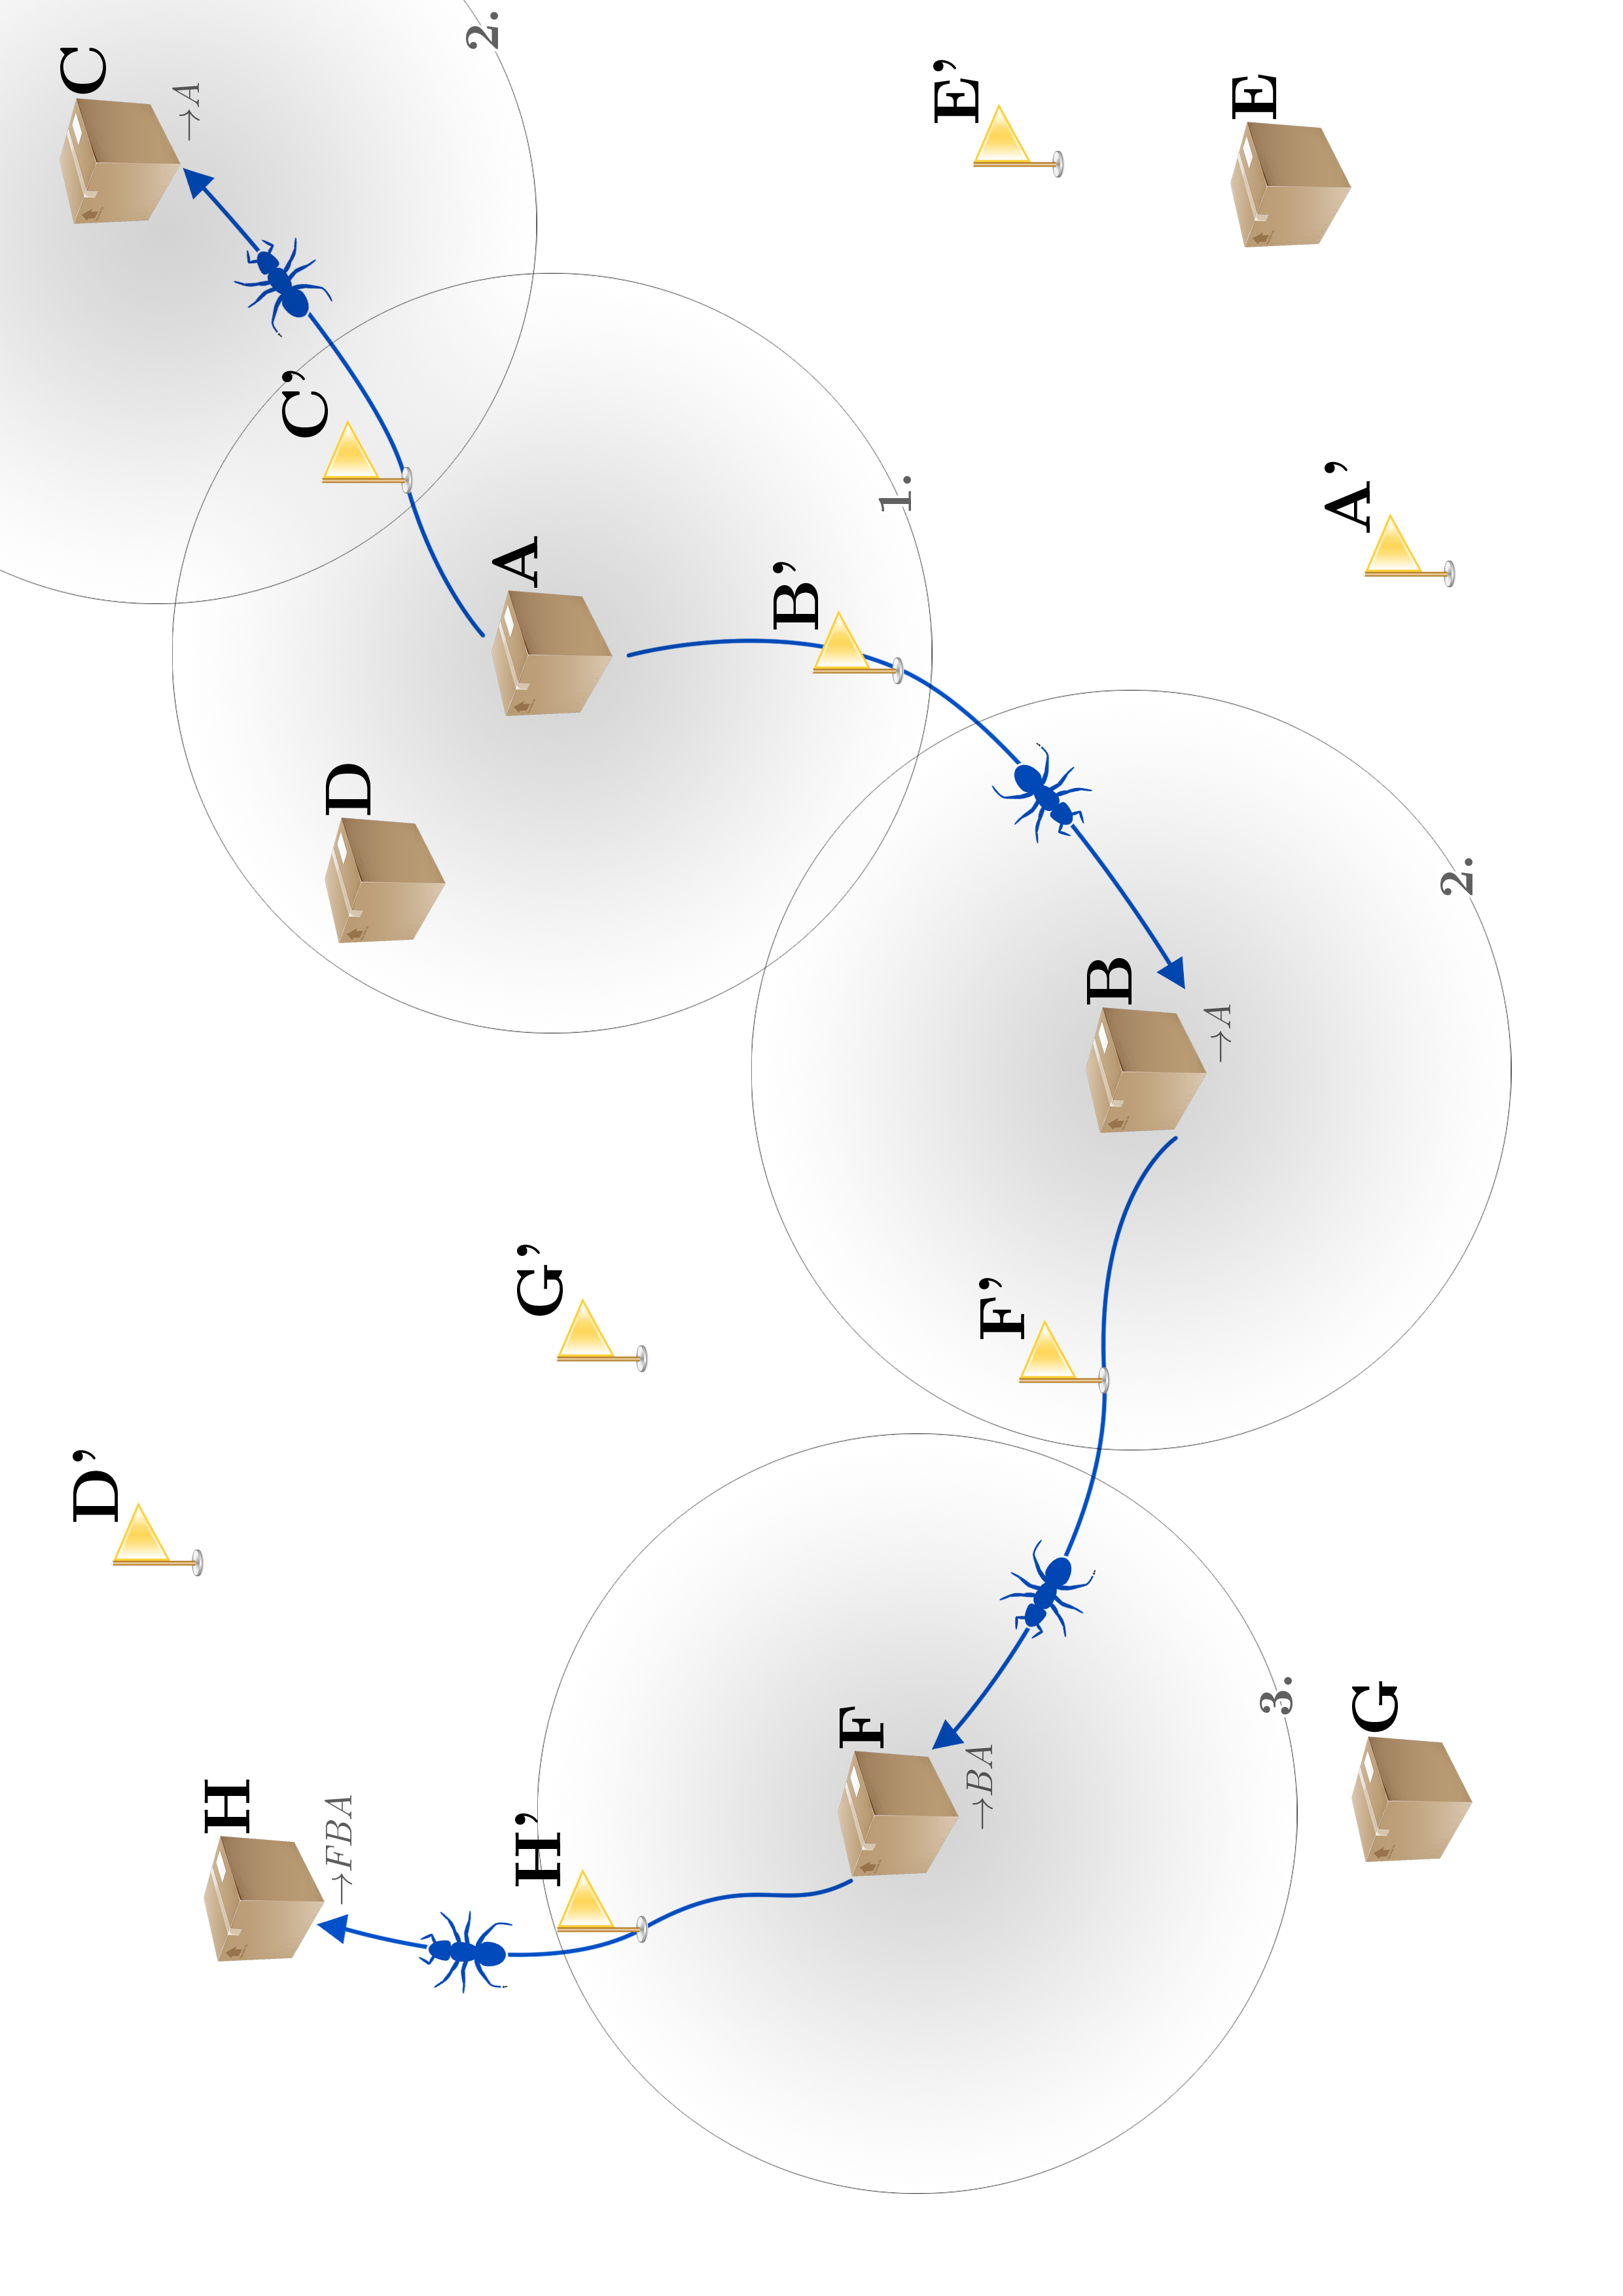
\includegraphics[width = 0.90\textwidth]{./figs/feasibility.png}}
		\end{center}
		\caption{Example Scenario I (\ref{subsec:scenario1})}
		\label{Fig:scenario1}
        \vspace{0.5pt}
\end{figure}

\begin{figure}[!h]
        \vspace{0.5pt}
        \begin{center}
       			\setlength\fboxsep{0.5pt}
				\setlength\fboxrule{0.5pt}
                \fbox{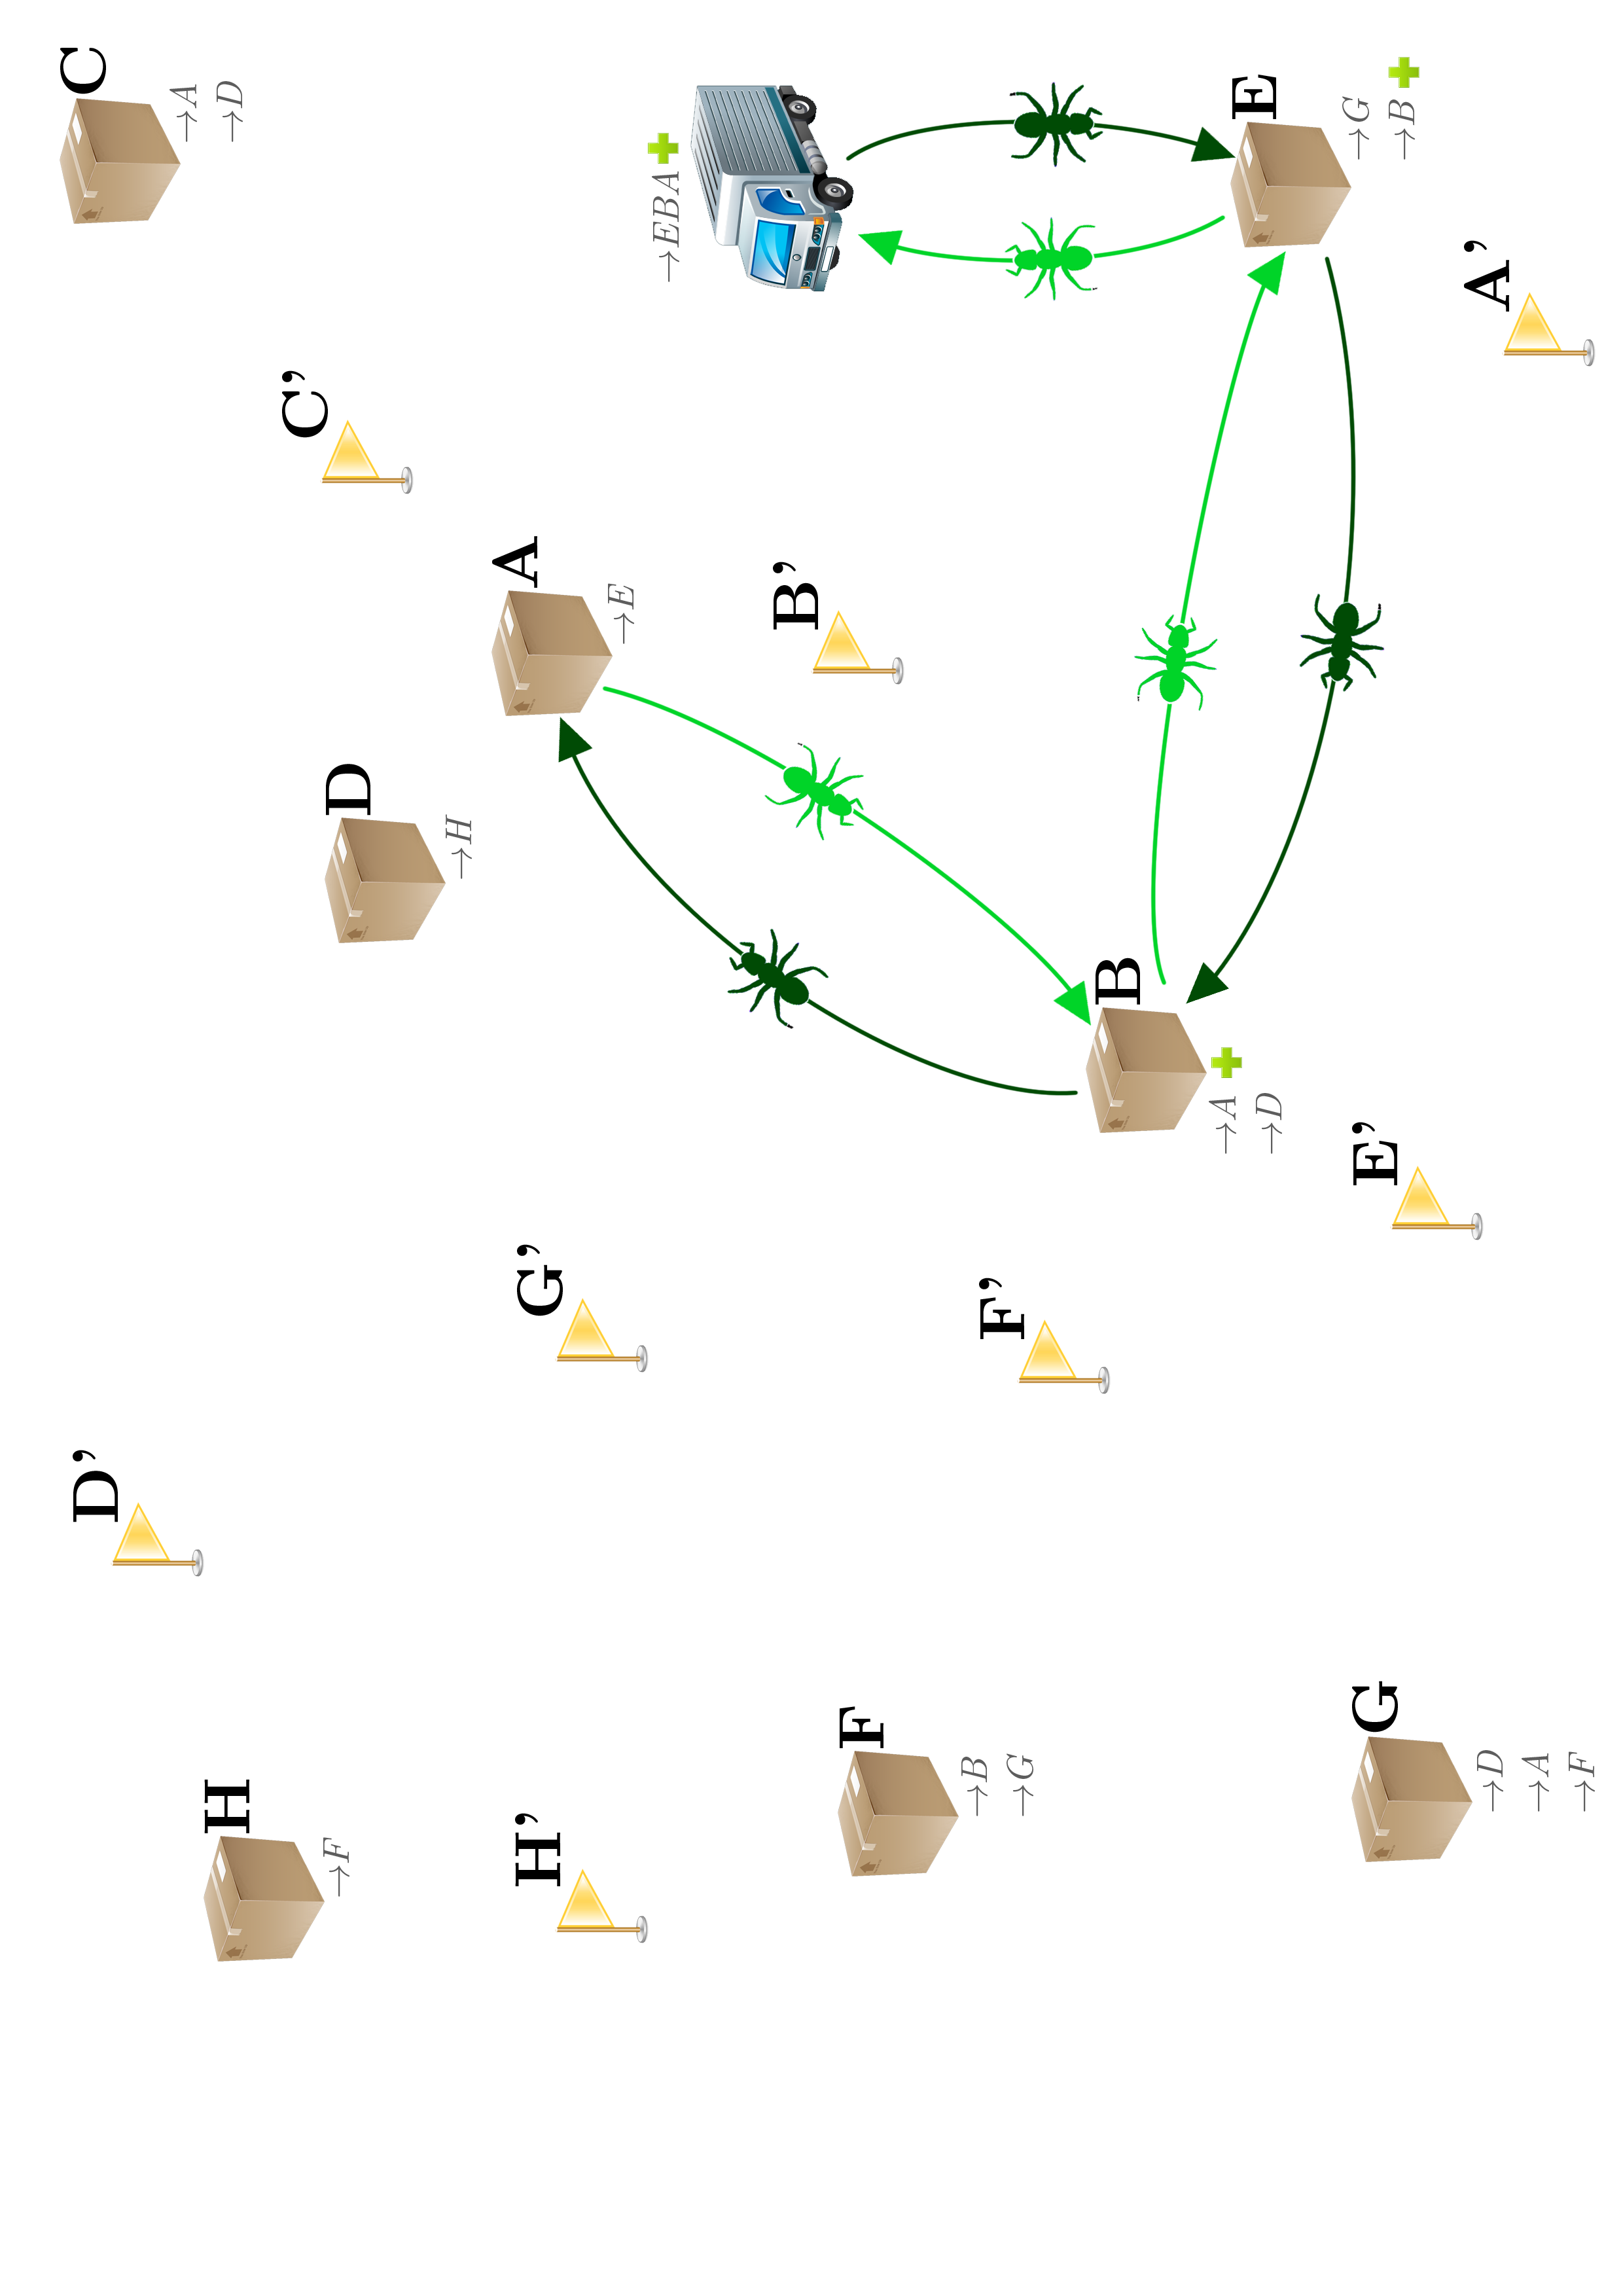
\includegraphics[width = 0.90\textwidth]{./figs/exploration.png}}
		\end{center}
		\caption{Exploration Ants (example scenario 2)}
		\label{Fig:Radios}
        \vspace{0.5pt}
\end{figure}

\begin{figure}[!h]
        \vspace{0.5pt}
        \begin{center}
       			\setlength\fboxsep{0.5pt}
				\setlength\fboxrule{0.5pt}
                \fbox{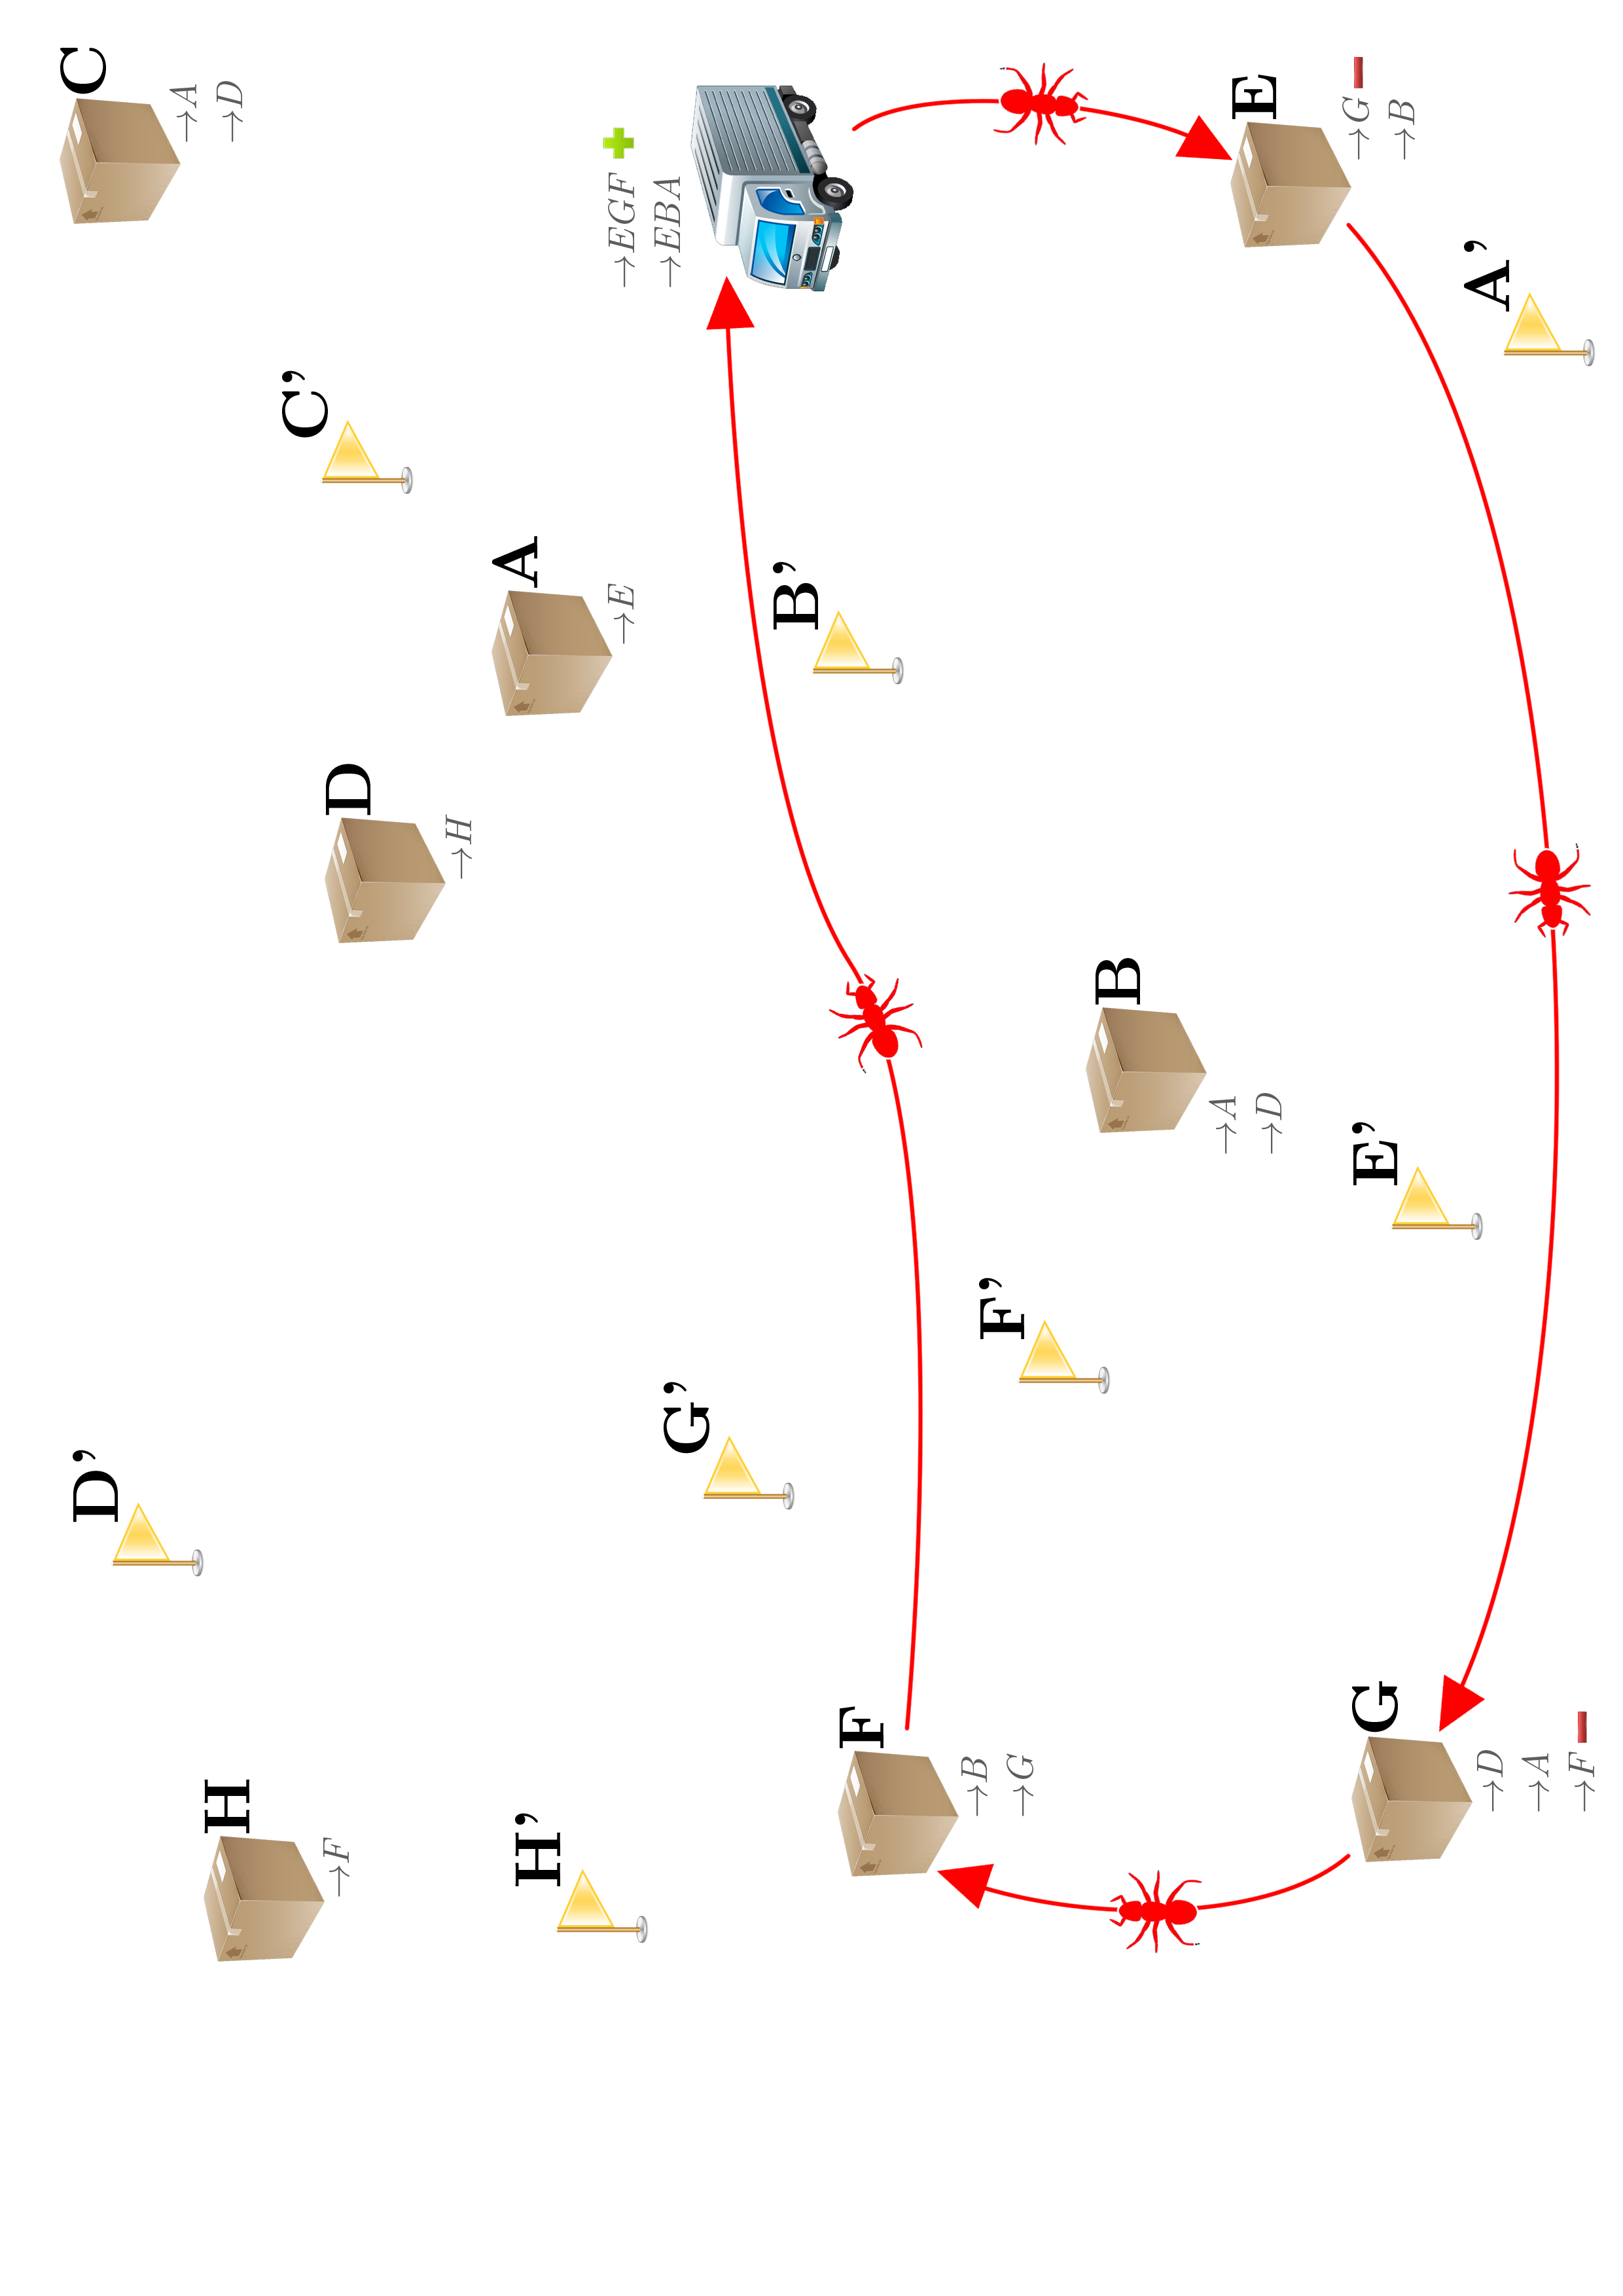
\includegraphics[width = 0.90\textwidth]{./figs/intention.png}}
		\end{center}
		\caption{Intention Ants (example scenario 3)}
		\label{Fig:Radios}
        \vspace{0.5pt}
\end{figure}
